%!TEX root = ../main.tex

\chapter{Music and listening}
\label{ch:3}

In Chapter \ref{ch:2}, we went over methodological limitations in previous research on MECs, and outlined a set open issues based on the reviewed literature. The present chapter introduces a study following some of the recommendations laid out in Chapter \ref{ch:2}, in which the relationships between MECs, piloerection, pleasure, musical content, stylistic preference, familiarity, and liking are examined in a controlled, longitudinal experiment.

\section{Introduction}

Broadly speaking, the present study aimed to investigate the effects of three independent variables (musical content, stylistic preference, and familiarity) on three dependent variables (MECs, piloerection, and pleasure), as well as the extent to which static ratings of liking for pieces of music could be predicted by all of these factors combined.

\emph{Musical content} here refers to the collection of stimulus-driven characteristics that might influence the propensity of a specific piece of music to induce MECs. As discussed in Chapter \ref{ch:2}, MECs have previously been considered to be highly idiosyncratic. There is merit to this claim, given that in many studies, one participant's MECs-inducing stimulus is successfully used as another participant's control stimulus. However, this view is incompatible with the fact that there is evidence (though mostly correlational in nature) for an association between MECs and a range of clearly defined acoustic and musical elicitors, which should logically lead to some pieces of music being more likely to induce MECs than others. It is unlikely that a specific combination of elicitors always induces MECs for everyone, or conversely, that MECs can be experienced when listening to any piece of music. Instead, we would expect that, in aggregate, pieces of music which induce MECs for some people are more likely to induce MECs in others than randomly selected pieces of music.

A possible way to establish causation for this claim is to assess the occurrence of MECs when listening to tracks that have previously been reported to elicit MECs compared to tracks that have not. The possibility of confounding factors can be limited by matching this second set of tracks with the first as closely as possible on every parameter (including, in this case, artist, duration, and popularity) except musical content, resulting in two comparable pools of tracks (hereafter referred to as \emph{sources}). While it is likely that some tracks from the matched source also have the ability to cause MECs, we would expect tracks from the chills source (i.e., tracks previously reported to elicit MECs) to cause more MECs (see Chapter \ref{ch:4} for a more thorough discussion of the assumptions behind this study design). When it comes to musical content, the hypothesis was therefore that tracks which cause MECs for some people are more likely to cause MECs for other people. Causal evidence from this study should help clarify if this is the case, which would suggest that there is a clear effect of acoustic and musical elicitors on the occurrence of MECs, or if MECs can be experienced when listening to any music, which would suggest that they are an indicator of individualised responses to music, or at least that other factors are involved.

\emph{Stylistic preference} and \emph{familiarity} are two of these factors (included in the \emph{listening context} section of the model of MECs introduced in Chapter \ref{ch:2}), and are likely to be involved either way, considering that the occurrence of MECs is not determined by stimulus-driven properties alone. Previous research identified conflicting effects of stylistic preference \parencite{bannister2018, nusbaum2011}, but these findings were limited in two ways. First, the hypothesis was that the occurrence of MECs might be driven by preference for a specific subset of musical genres, resulting in findings that individuals who experience MECs tend to prefer reflective and complex genres in one study \parencite{bannister2018}, or upbeat and conventional genres in the other \parencite{nusbaum2011} as measured by STOMP, the Short Test Of Music Preferences \parencite{rentfrow2003}. However, if MECs involve an interaction between listener, context, and music (see Chapter \ref{ch:2}), we would expect an individual's stylistic preference for any genre to have an effect on the occurrence of MECs. In other words, rather than the characteristics of specific genres leading to more MECs, stylistic preference should drive the occurrence of MECs by making them more likely to occur in an individual's preferred genre, through a combination of personal taste and stylistic enculturation, possibly linked with an effect of expectation on MECs \parencite[see][]{beier2020}. 

Second, there are limitations to the methods that were used to assess stylistic preference. STOMP was designed to investigate personality differences in the preference for specific musical genres, and consists of asking participants to provide Likert scale preference ratings for 14 genres. More recent approaches require participants to rate their preference for musical exemplars assigned to each genre, instead of rating labelled genres directly \parencite{bonnevilleroussy2017,rentfrow2011}. Such approaches are limited because they all rely of some degree of reductionism and subjective interpretation in genre labelling and categorisation (by participants or researchers), which is therefore not consistent across individuals, and because most adults have omnivorous stylistic preferences \parencite[for a review, see][]{greasley2016}. For the purpose of the present study, this issue was circumvented by directly asking participants whether a given track was in a liked genre or not, without relying on labelling said genre, allowing for an objective and causal investigation of the hypothesis that more MECs are experienced when listening to tracks in preferred musical genres.

\emph{Familiarity}, similarly to stylistic preference, could possibly affect the occurrence of MECs. There is a long history of research on the link between familiarity and liking, including seminal work such as Zajonc's (\citeyear{zajonc1968}) mere exposure effect and Berlyne's (\citeyear{berlyne1971}) inverted-U relationship. Overall, previous research identified a strong relationship between familiarity and liking for music \parencite[for a review, see][]{greasley2016}. Of relevance to research on MECs, familiarity was even identified as more important than liking for emotional engagement with music \parencite{pereira2011}. When it comes to direct empirical evidence of an association between familiarity and MECs, however, results are mixed and were affected by methodological limitations, as discussed in Chapter \ref{ch:2}. Notably, repeated exposure was only assessed in the context of a single experimental session \parencite{baltes2011,bannister2020b,blood2001} or over a longer period, but for a single participant \parencite{grewe2007}, or the effect of familiarity was only assessed statically, by comparing ratings of familiarity across stimuli (see Chapter \ref{ch:2}). Longitudinal methods have been underused in research on familiarity and liking \parencite{greasley2016}, but they remain the best way to systematically manipulate familiarity in order to show causal effects on MECs. The present study used such an approach, with the hypothesis that increased exposure, and therefore familiarity, results in increased occurrences of MECs.

In terms of dependent variables, the present study examined all of MECs, piloerection, and pleasure. The reasons for considering different dependent variables instead of MECs only were threefold, and are all discussed in Chapter \ref{ch:2}. First, not all MECs are accompanied by piloerection, so there is a need to investigate whether MECs and piloerection are similarly affected by changes in track source, stylistic preference, and familiarity. Second, while there is a documented association between MECs and pleasure, there have been few attempts, if any, to disambiguate the two responses in previous research. Finally, while the use of objective measures would have been preferred, such as the automatic detection of piloerection, we have argued that a combination of self-reports and objective measures is currently best suited for the study of MECs. Collecting data on these three variables therefore allowed us to explore the hypotheses that piloerection overlaps with self-reported MECs, and that MECs are more likely to occur in musical passages perceived as pleasurable.

The research design for this study aimed to provide ways to systematically manipulate all three independent variables, while also following the methodological recommendations laid out in Chapter \ref{ch:2}, which argue for the use of naturalistic listening experiences using existing pieces of music in order to increase ecological validity, which are both considered crucial when investigating aesthetic and emotional responses to music \parencite{eerola2018,hargreaves2010, hodges2016}. In summary, the main hypotheses underlying this study were that the occurrence of MECs increases for tracks previously identified to cause MECs (as discussed above), with stylistic preference, and with familiarity (both included as hypotheses of interest in Chapter \ref{ch:2}), that there is an overlap between piloerection, MECs, and pleasure in music (as discussed in the previous paragraph), and that the combination of all of these factors has an effect on overall liking for pieces of music (a key motivation for the present thesis).

\section{Methods}

\subsection{Stimulus selection}

\subsubsection{Online survey}

We conducted a survey study hosted on Qualtrics (Qualtrics, Provo, UT) with several distinct objectives: 1) build a set of ecologically valid stimuli from a single, controlled, and contemporary source for the purpose of the present study, 2) build a large dataset of onset of MECs for the computational analysis detailed in Chapter \ref{ch:5}, 3) collect some basic demographic information for further investigation into the effects of individual differences on the occurrence of MECs, and 4) contribute to building a pool of potential participants for the present study. This survey was conducted online in order to access a wider and more representative sample of the population.

Survey responders were asked to report basic demographic information such as age, gender, and country of residence. They were then asked to provide up to ten pieces of music that include instants at which they often experience chills (defined here as shivers, goosebumps, or a tingling sensation experienced in response to music listening). For each piece of music, participants were asked to provide the name of the artist or composer, the title of the piece of music, a link where the piece of music can be streamed online (on Youtube, Spotify, SoundCloud, or a similar platform), and at least one and up to five precise timestamps for instants at which they often experience the onset of chills (i.e., the exact moment at which chills tend to begin). Participants were advised not to include music which can be strongly associated with specific personal memories, such as life events (e.g., a wedding, a memorable concert, etc.) or periods of time (e.g., summer of 2013, secondary school, etc.), or music that was taken from a film soundtrack if they had watched the film in question. These restrictions, taken from a previous study by \textcite{salimpoor2009}, were meant to maximise the possibilities that the MECs in question were induced by widespread and detectable acoustic and musical elicitors, as opposed to autobiographical elicitors driven by episodic memory, which would not generalise across participants.

Survey responses for the present study were collected between February 2018 and May 2018, although the survey was left running for longer to collect more onsets of MECs for the computational study presented in Chapter \ref{ch:5}. The questionnaire was disseminated on a wide range of online platforms, including international academic mailing lists, staff and student mailing lists within Queen Mary University of London, as well as Twitter\footnote{\url{https://www.twitter.com}} and Reddit.\footnote{\url{https://www.reddit.com}} Complete responses were collected from 221 participants, ranging in age from 18 to 77 years (\emph{M} = 25.3 years, \emph{SD} = 9.4 years). Of the participants who reported their gender, 72 identified as female and 144 as male. Responses originated from a wide range of geographical areas (50 \% North America, 37\% Europe, 5\% Asia, 5\% Oceania, 2\% South America, 1\% Africa). The resulting data required some manual cleaning, consisting of removing entries which were not changed from the default answers provided in the survey, as well as discarding non-valid URLs. This process resulted in retaining 214 complete responses, corresponding to 671 tracks.

From these 671 tracks, we needed to subset a pool of suitable stimuli according to the requirements of the study. This process involved four steps. First, tracks which were not available for streaming on Spotify were discarded. Second, tracks which were longer than five minutes in duration were discarded (with a few exceptions discussed later), in order to keep the duration of the experiment manageable, considering that the participants would need to listen to several tracks many times throughout the lab experiments and the longitudinal phase of the study. This duration is consistent with similar studies requiring participants to listen to several tracks in one sitting \parencite{laeng2016,mori2014b}, and was preferred to selecting excerpts from each track \parencite{blood2001,sachs2016,salimpoor2009}, so as to ensure ecological validity by allowing participants to listen to tracks in full. Third, tracks for which MECs were reported within ten seconds of the beginning or the end of the track were discarded. This threshold was set arbitrarily, with the objective to maximise the chances of new listeners experiencing MECs. Finally, tracks for which MECs were reported within ten seconds of any passage including sung lyrics were discarded. It was decided to implement this restriction because sung lyrics have the potential to introduce additional confounding factors. This is often accounted for in previous research by asking participants to provide instrumental music only, but we felt this was overly restrictive for the purpose of the present study. These thresholds (five minutes for track duration and ten seconds for buffers between reported MECs and track beginning, end, and sung lyrics) were chosen by comparing different threshold values in order to retain an adequate number of tracks while minimising track duration and maximising buffers.

This process results in a pool of 93 tracks, which we subsequently refer to as tracks from the \emph{chills source}.

\subsubsection{Matching procedure}

As discussed above, a part of the experimental design for this study relied on comparing tracks previously reported to cause MECs to tracks that were not, matched as closely as possible on every parameter except musical content, resulting in two comparable pools of tracks. The rationale behind this manipulation was that, considering that acoustic and musical elicitors of MECs have been identified in previous research, it logically follows that some pieces of music should include more of these elicitors than others. If the hypothesis that, as a consequence, music which induces MECs for some people is more likely to induce MECs in others, tracks from the chills source should then be more likely to induce MECs than tracks from the matched source. This reasoning is central to several experiments in the present thesis, and the assumptions and limitations behind it are covered in more detail in Chapter \ref{ch:4}.

The matching procedure used in this study was inspired by the one used by \textcite{jakubowski2017}. In their study, the authors aimed to obtain close matches for a set of 100 tracks that were named as causing involuntary musical imagery (otherwise known as earworms) in order to run statistical comparisons between both sets of tracks. Matching was performed by identifying a pool of candidate tracks with similar artists, time periods, chart positions, and genres as the target set of tracks. Matching was then conducted algorithmically, allowing precise matching on several variables at once: artist, genre, and chart information (highest entry, longevity, and days since exit).

While the procedure for the present study was conducted manually, a similar algorithmic procedure is detailed in Chapter \ref{ch:4}. In the present study, each track from the chills source received five candidates for matches, which were manually shortlisted in the following way. First, a match should not have been mentioned in any of the survey responses as a track which can elicit MECs. Second, a match should be from the same artist as the target track. Third, its duration should be between 2.5 and 5 minutes. Fourth, its popularity, as assessed by the number of plays on Spotify, should be between half and double that of the target track. Finally, when possible, it should be sourced from the same album as the target track. If not, search should be expanded to tracks produced as close as possible in time to the target track. This process allowed to select candidate tracks while controlling as much as possible for stylistic preference (following the assumption that artists tend to produce tracks in relatively closely related genres), duration (in order to allow for similar opportunities to experience MECs), and quality (using popularity as a proxy for this more abstract measure). Each candidate track was ranked manually, resulting in subjective rankings of how closely related they were to their target track.

The top three matches for each track were retained, resulting in a pool of 279 tracks, which we subsequently refer to as tracks from the \emph{matched source}.

\subsection{Software and device}

\subsubsection{Stimulus allocation}

The objective of the stimulus allocation online session was to select an individual stimulus set of 20 unfamiliar tracks for each participant, consisting of five tracks for each combination of source (chills or matched) and stylistic preference (liked or disliked). This set of tracks would then be used by this participant for the rest of the study.

Unfamiliarity was key to the present study, so there was a need to limit exposure to each track as much as possible before the first lab session. In order to do so, short excerpts were extracted for each track. The duration of said excerpts was decided based on previous research. While the valence of a piece of music can generally be recognised in excerpts lasting as little as one-eighth of a second \parencite[for a review, see][]{mace2012}, it generally takes up to a second to identify the genre of a piece of music \parencite{gjerdingen2008,mace2012}. When it comes to familiarity or song recognition, however, estimates vary between less than a second and up to ten seconds \parencite{jensenius2002,krumhansl2010,pereira2011,schellenberg1999}, with the added caveat that salient features are required \parencite{jensenius2002}, such as dynamic, high-frequency spectral information \parencite{schellenberg1999}. To minimise the likelihood of familiar tracks being selected for the first lab session, we opted for an excerpt duration of 15 seconds, which we deemed short enough to not affect the outcomes of the present study while safely allowing participants to recognise both familiarity and stylistic preference for a given track.

There is much less information available about which excerpt should be sampled from all possible excerpts present within a track, with \textcite{mace2012} reporting random samples taken between 00:30 and 04:00 for each track, and other authors simply not reporting that information \parencite[e.g.,][]{bonnevilleroussy2017,krumhansl2010,pereira2011}. Randomly selecting excerpts felt inadequate, so we opted for the heuristic of choosing the loudest moment for each track as long as it didn't correspond to a previously reported onset of MECs, following previous recommendation about salience and dynamics \parencite{jensenius2002,schellenberg1999}, and assuming that this would often correspond to the most recognisable moment of a track. More precisely, each track was trimmed by 10\% in duration on each side, and a moving average of absolute amplitude was computed using a 15-second sliding window. A 15-second excerpt centred around the peak of the moving average was selected for each track, as long as no onsets of MECs were reported during or within five seconds of the excerpt. If MECs were previously reported near the excerpt, the process was repeated using each following peak in average amplitude until a suitable excerpt was identified for each track. A one-second fade in and fade out was applied to each excerpt, before applying Root Mean Square (RMS) normalisation to harmonise loudness between excerpts, and exporting the excerpts to MP3 format at 170--210 kbps to reduce loading times during the online session. Audio computations and manipulations were conducted using the \emph{tuneR} \parencite{ligges2018} and \emph{seewave} \parencite{sueur2008} R packages, and RMS normalisation and MP3 exports were executed with Audacity.\footnote{\url{https://www.audacityteam.org}}

Each excerpt from the chills source was also tagged with a genre, with its associated excerpts from the matched source inheriting that tag. Note that this procedure still circumvented issues of genre labelling when determining stylistic preference, since these genre tags were only used to group excerpts into broadly similar categories in order to more quickly hone in on an ideal set of stimuli for each participant, as described in the next paragraph. Excerpts from the chills source were tagged with genre labels taken from MG-CT, the Music Genre-Clips Test \parencite{bonnevilleroussy2017}, by manually comparing the excerpts from the present study to the excerpts provided by the MG-CT and selecting the most closely related genre, resulting in excerpts being categorised into 11 different genres, ranging from two excerpts for punk music to 28 excerpts for classical music.

The online questionnaire for the stimulus allocation session was developed using \emph{psychTestR} \parencite{harrison2020}, an R package allowing for the design of online experiments recruiting a more complex internal logic, using R code snippets, than that provided by most online survey platforms. The questionnaire was hosted on shinyapps.io,\footnote{\url{https://www.shinyapps.io}} and participant data was automatically uploaded to Dropbox\footnote{\url{https://www.dropbox.com}} upon completion. Using psychTestR was necessary to dynamically adapt the order of the presented excerpts in order to select a set of 20 appropriate stimuli as fast as possible, since it was not reasonable to expect participants to listen to and provide ratings for all 372 available excerpts before making a selection. When taking the questionnaire, participants were first asked for their age and gender, before taking the Musical Training sub-scale of the Gold-MSI \parencite{mullensiefen2014}. They were then presented with the stimulus allocation task. For this task, participants were presented with a series of excerpts and posed two questions for each excerpt, asking them to report whether or not they knew the piece of music the excerpt was taken from (with a possibility to answer that they were unsure), and to rate how much they tended to like music which sounded like the excerpt on a five-point Likert scale ranging from ``Dislike very much'' to ``Like very much''. In the instructions before the test, participants were explicitly instructed that the second question referred to the genre or style of the excerpt, and that they were not asked whether or not they liked the excerpt itself. 

The goal of the task was to select five unfamiliar excerpts for each combination of source (chills or matched) and stylistic preference (liked or disliked), while maximising the number of extreme values for stylistic preference (i.e., ``Dislike very much'' or ``Like very much''). In order to do so, the order of presentation of the excerpts was determined using the following logic. First, two excerpts were sampled from the chills source for each tagged genre, and presented in a random order. If excerpts were familiar or familiarity was unsure, they were discarded. If excerpts were unfamiliar and rated with extreme values of stylistic preference, they were retained. Stylistic preference of the presented excerpts was averaged by genre and updated with each answer, allowing the questionnaire to identify the most liked and disliked genres for a given participant at any time. Then, more excerpts from the chills source were played, focusing on the most liked or disliked genres depending on which category had the fewest retained excerpts, in order to maintain the balance between the number of excerpts in very liked and disliked genres. Once 40 excerpts were played, ten excerpts were retained for both liked and disliked genres, and were locked in for the chills set, even if they gathered less extreme ratings, e.g., ``Dislike somewhat'' instead of ``Dislike very much''. Then, the task randomly iterated through the excerpts from the matched source that were paired with each retained excerpt, to try to identify similarly liked or disliked matches, starting with the most highly ranked match before trying the other two matches. Similarly, excerpts from the matched source were discarded if familiar or if familiarity was unsure, and were retained if they were unfamiliar and had extreme ratings of stylistic preference in the same direction as their associated excerpt from the chills source. If enough liked or disliked excerpts were retained, the task stopped trying to fill that category of stylistic preference. The task ended successfully if each combination of source and stylistic preference received five excerpts with extreme ratings of stylistic preference, or if 80 excerpts were played and excerpts with non-neutral ratings of stylistic preference could be allocated to each condition. Participants failed the task if it ran out of excerpts from the matched source, or if 80 excerpts were played and five excerpts could not be allocated to each condition.

\subsubsection{Goosecam}

Before describing the software used for the lab sessions, it is useful at this point to discuss the device that was used to record piloerection during these sessions. The device consisted of a slightly more compact Goosecam (see Chapter \ref{ch:2} for a brief description), intended to minimise the discomfort of wearing the rather bulky original version of the Goosecam, made of a 160 $\times$ 40 $\times$ 40 mm aluminium bar with a cutout to accommodate a webcam \parencite{benedek2010}. The thorough specifications detailed by \textcite{benedek2010} allowed for the design of a smaller device which complied with the original requirements of filming the skin through a 40 $\times$ 40 mm cutout, illuminated from an angle of approximately 15º, from a distance of 46 mm. The body of the device was made of a laser-cut box using a 3 mm acrylic sheet, the inside of which was lined with matte black self-adhesive vinyl to minimise reflections. The pattern for that box was adapted from an open-source Raspberry Pi case pattern,\footnote{\url{https://github.com/diy-electronics/raspberrypi-b-plus-case}} and is shown in \autoref{fig:con-1}.

\begin{figure}[t!]
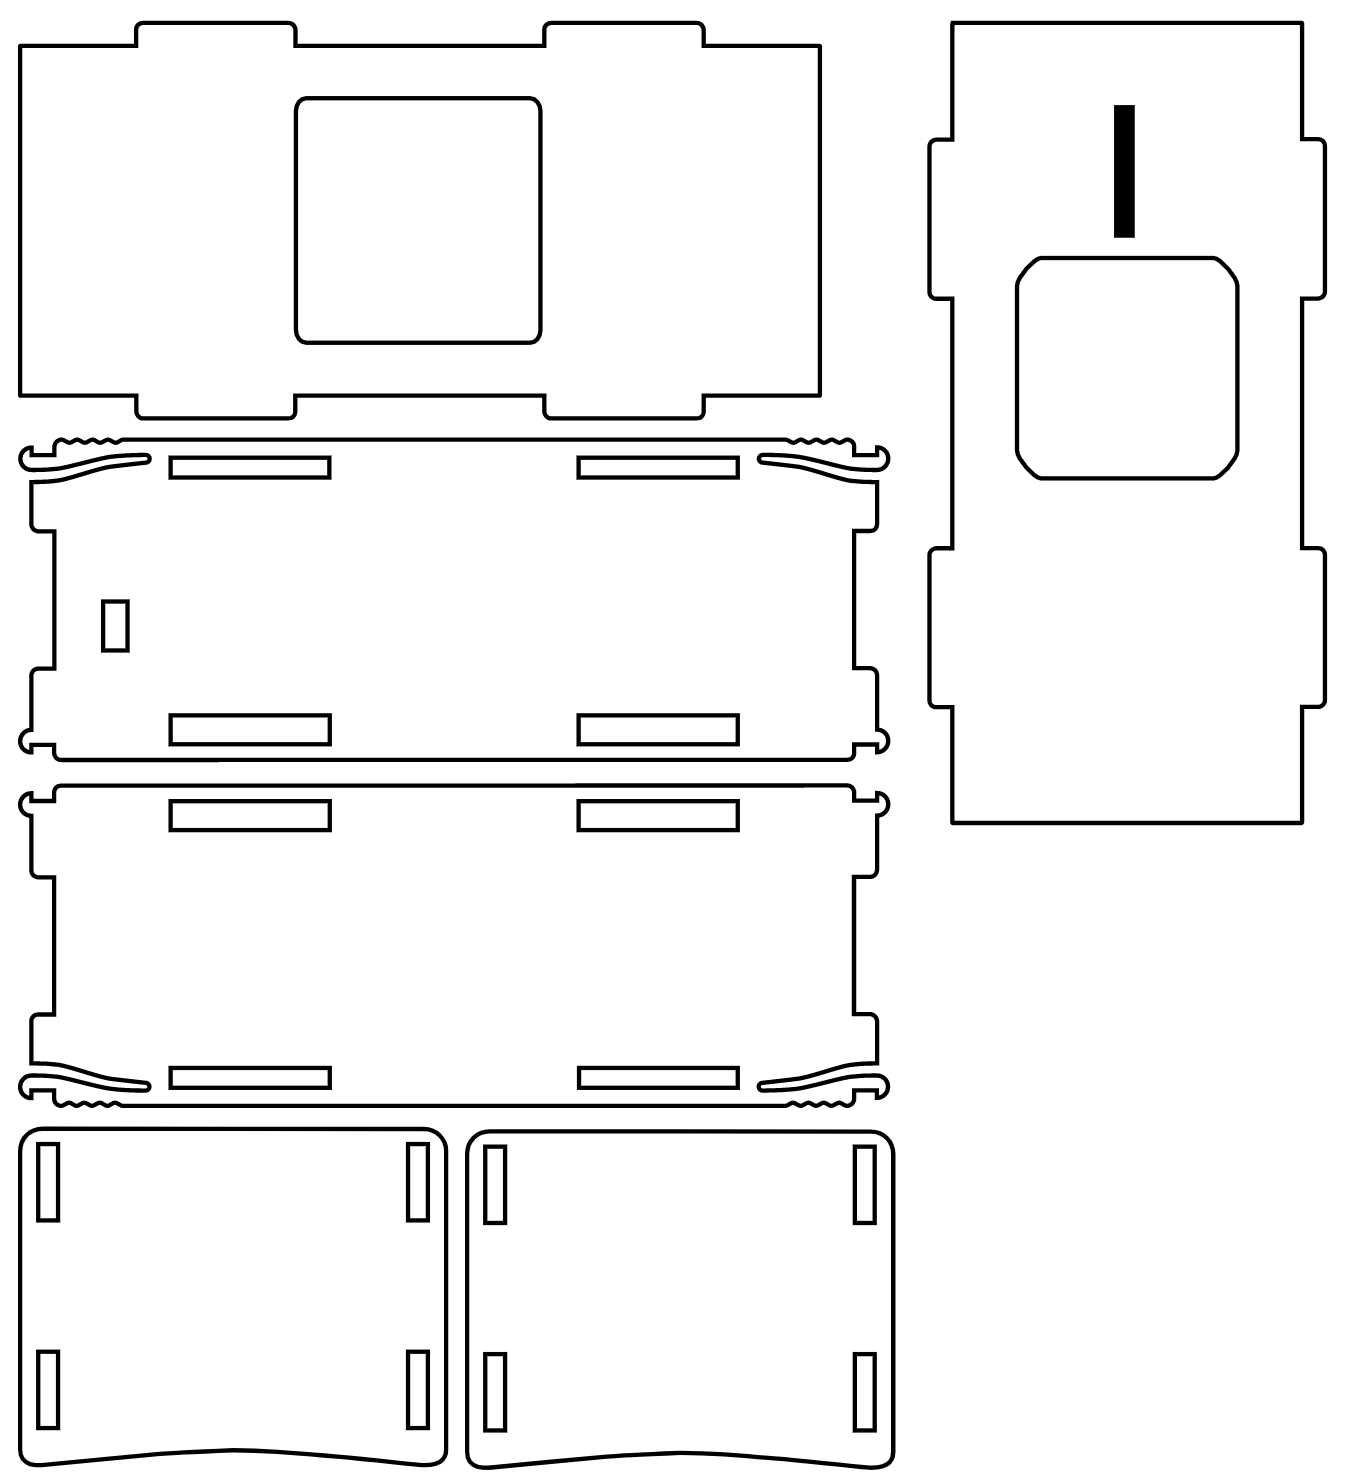
\includegraphics[width=\textwidth]{con-1.png}
\centering
\caption{Laser-cut vector design for the compact Goosecam. The top panel shows the bottom side of the device, with a cutout for the skin to show through. The two panels below that show the long sides of the device, with pressure-activated locking mechanisms, cutouts for the top and bottom panels, and a cutout for the cable connecting to the Arduino board. The two bottom panels show the short sides of the device, with cutouts for the locking mechanisms. Finally, the panel on the right shows the top side of the device, with a cutout for the GoPro camera, and a groove in black for the camera mount.}
\label{fig:con-1}
\end{figure}

Inside the Goosecam, various components were powered and controlled by an Arduino Nano board: a white LED panel affixed to one of the sides of the body to provide directional light at an angle from the skin, a small OLED display to facilitate stimulus identification when processing the videos for the analysis, and a piezo buzzer and a green LED light to enable precise synchronisation between the video and audio signals. All of these components were kept in place with a healthy amount of hot glue to ensure they would not get in between the camera and the skin cutout. The camera for this version of the Goosecam was a GoPro Hero5 Session---a compact camera which allows native linear correction for the fisheye distortion that is common in many GoPro cameras. Finally, the edges of the bottom side of the box were padded with foam sheet to minimise participant discomfort, and the device was held in place by elastic velcro straps looped through the bottom cutouts of the side panels (see \autoref{fig:con-2}).

\begin{figure}[t!]
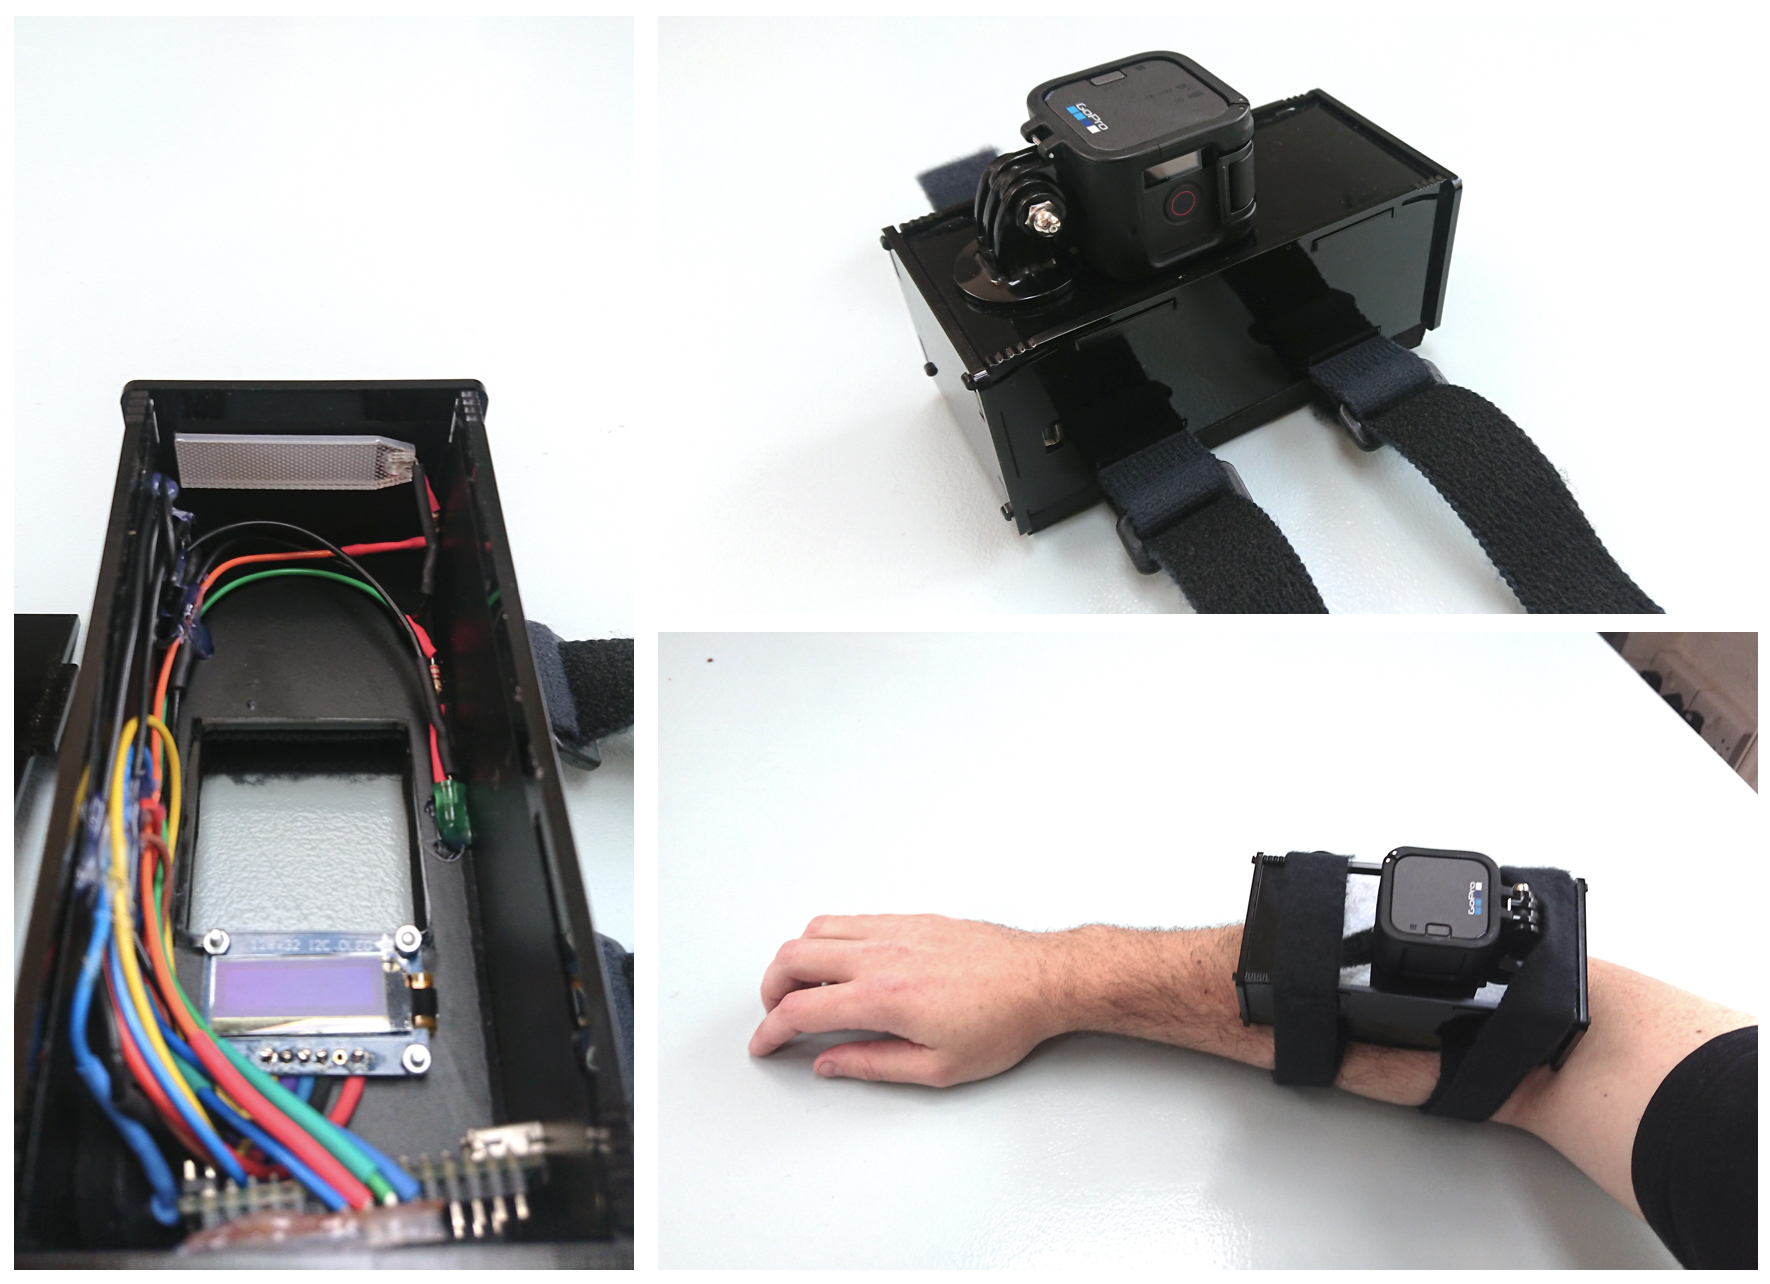
\includegraphics[width=\textwidth]{con-2.jpg}
\centering
\caption{Pictures of the compact Goosecam. The picture on the left shows the internal components with, going top-down, the white LED panel, the green LED, the OLED display, the piezo buzzer hidden in the bottom-left corner, and the Arduino board. The other two pictures show the Goosecam with the GoPro mounted on top.}
\label{fig:con-2}
\end{figure}

An Arduino script controlled the board. It read data sent from the computer it was connected to via the board's serial port, and extracted from this data information about whether a track was about to start playing or had just stopped playing, as well as unique identifiers for participants, lab sessions, and tracks. When a track started, the board instructed all indicators to switch on (white LED panel, LCD screen displaying all identifiers, green LED, and piezo buzzer). After one second, the components switched off except for the white LED panel which provided illumination for the skin. The panel switched off when a new serial message was received to indicate that a track had just ended.

\subsubsection{Lab session platform}

The objective of the first and last lab sessions was to collect continuous data as participants listened to full tracks. We were interested in gathering piloerection data, acquired via the Goosecam, as well as continuous self-reports for the occurrence of MECs and pleasure. While it would have been interesting to record self-reports of MECs intensity (using a slider, for instance) in conjunction with piloerection data, in order to evaluate whether or not piloerection occurs beyond a specific threshold of MEC intensity (see Chapter \ref{ch:2}), it was decided to use button presses to record binary responses instead, for the purpose of the planned analyses and to minimise participant distraction given the complexity of the task.

The full tracks were converted to Ogg format with a 44.1 kHz sample rate and 16-bit bit depth, before RMS normalisation was applied using Audacity, with a target RMS level of -18 dB and linked stereo processing, ensuring that the original left/right stereo balance was maintained after normalisation. These steps were necessary to ensure consistent sound quality and levels when music was played at the same volume throughout the experiment \parencite{mori2014a}.

The platform for the lab sessions was designed using OpenSesame \parencite{mathot2012}, an open-source graphical experiment builder enabling the sequencing of graphical tasks based on code snippets written in Python. This platform was selected for its ability to record the precise timing of key strokes, and for the flexibility in its underlying logic and user interface design. The platform first presented participants with instructions about how to operate it, followed by a headphones volume calibration task, and a quick practice task (see \autoref{fig:con-3} for some of the instructions which were presented to the participants). The four actions participants were asked to take when listening to each track were to maintain the C key pressed down during experiences of MECs if any occurred, to maintain the M key pressed down whenever they found a musical passage pleasurable if at all, and after each track, to indicate whether or not they already knew the track they just listened to, and to rate how much they liked said track. The question about track familiarity was only presented in the first lab session, to confirm that the tracks were indeed unfamiliar following the online stimulus allocation task, and to present alternative tracks if not.

\begin{figure}[t!]
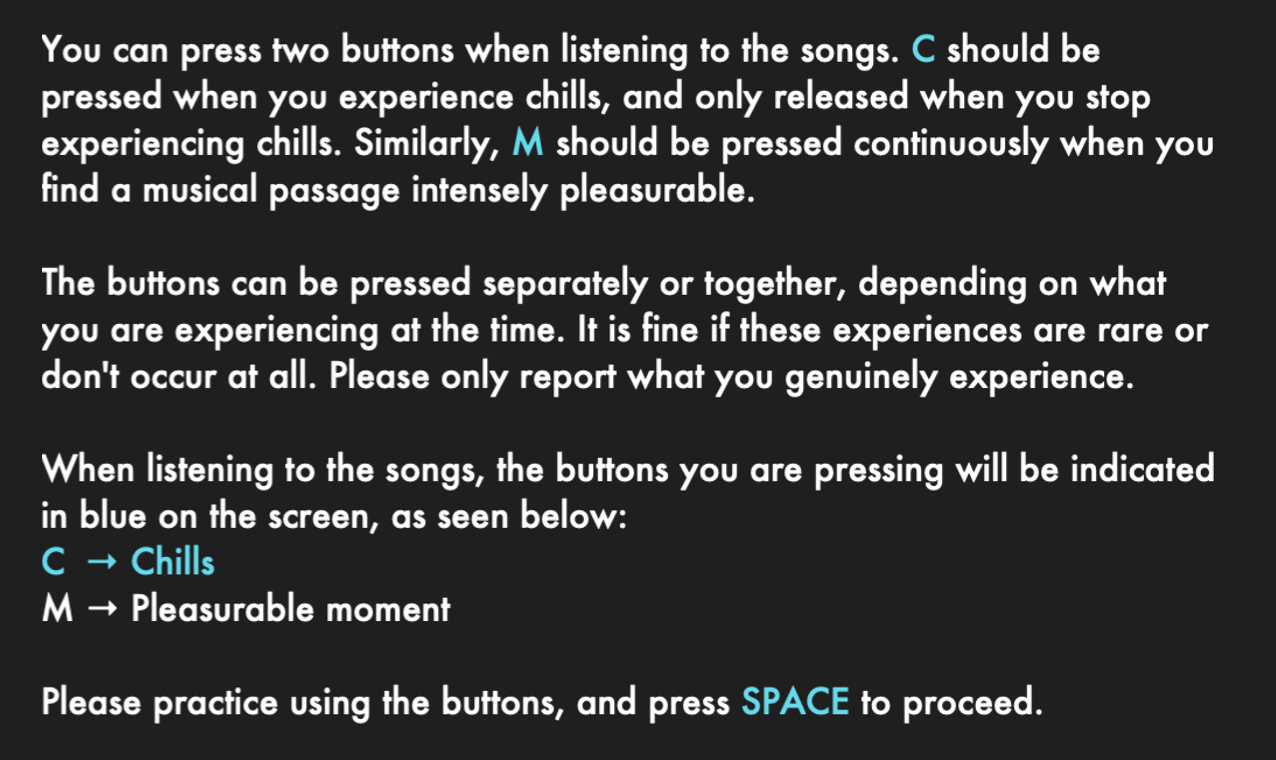
\includegraphics[width=\textwidth]{con-3.png}
\centering
\caption{Graphical user interface for the lab session platform. This step of the participant instructions describes how to use key presses to report occurrences of MECs and pleasure in music throughout the experiment. In this case, the C key is pressed down, and is therefore highlighted in blue in the user interface.}
\label{fig:con-3}
\end{figure}

For each track, the following series of actions and logging events were taken by the platform. First, a serial message was sent to the Goosecam one second before recording a 30-second baseline measurement (required for processing Goosecam data), concluded with another serial message to signify that the baseline recording was over. The platform then slept for three seconds, before reiterating the procedure and playing the track instead of performing a baseline recording (see \autoref{fig:con-4} to see the platform during baseline recordings and when playing a track). While the track was playing, the onset and offset of key strokes were precisely recorded, in order to log when and for how long participants reported occurrences of MECs or pleasure in music. The accuracy and synchronisation of serial messages, track-playing triggers, and key stroke logging actions were extensively tested and validated prior to running the experiment. Note that the potential effect of key presses on the occurrence of piloerection was not tested, due to extensive previous evidence that such an effect is most likely not present (see Chapter \ref{ch:2}).

\begin{figure}[t!]
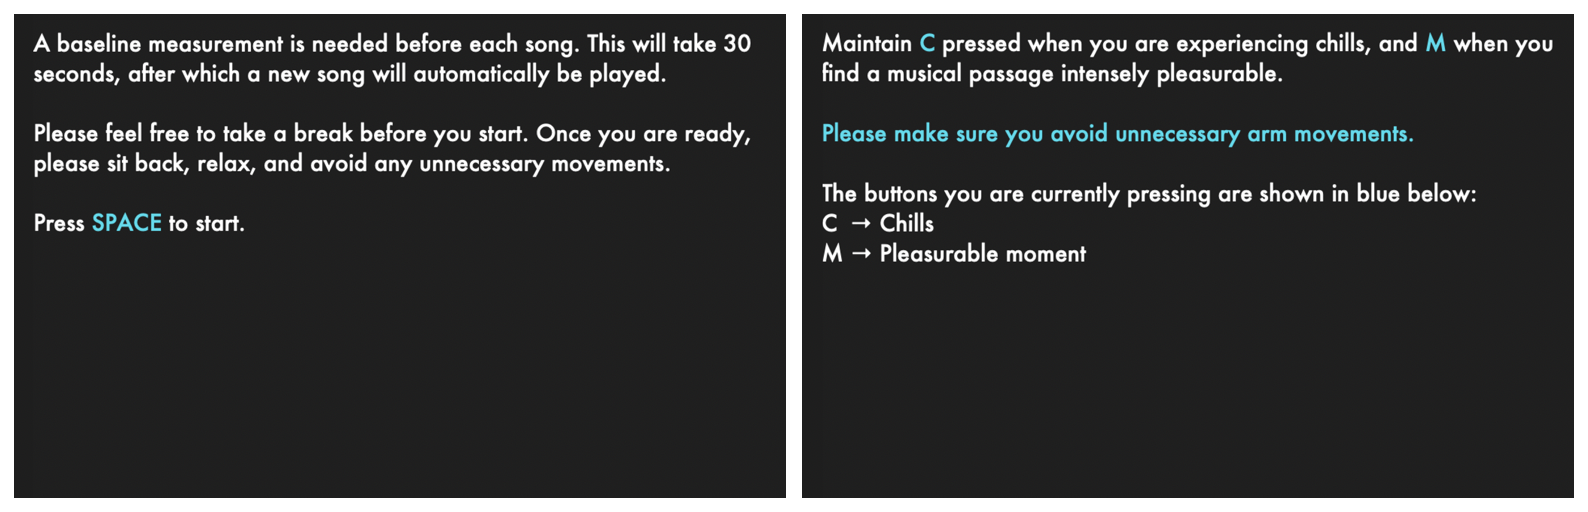
\includegraphics[width=\textwidth]{con-4.png}
\centering
\caption{Graphical user interface for the lab session platform during the track listening task. Before each track, a baseline recording is performed. During each track, participants can use key presses to report occurrences of MECs and pleasurable moments in music. During both phases, participants are instructed to avoid unnecessary moments.}
\label{fig:con-4}
\end{figure}

Similarly to the stimulus allocation task, the order of presentation of the tracks followed some underlying logic, aimed at ensuring that three unfamiliar tracks would be presented for each combination of source and stylistic preference, which is why five tracks per condition were retained in the stimulus allocation task to allow room for some of the retained track actually being familiar to the participants. In practice, for both high and low stylistic preference, the platform randomly selected three tracks from the chills source and their associated tracks from the matched source, and played them in random order. If a track was identified as familiar, it was discarded along with its paired track, and that pair was replaced by one of the two back-up options from the stimulus allocation task. The task ended successfully when the participant had listened to three unfamiliar tracks in each condition, or failed when no more tracks were available.

\subsection{Procedure}

Participants were recruited through internal mailing lists of undergraduate and postgraduate students at Queen Mary University of London, and by emailing the participants from the survey study who accepted to be contacted for future research. In order to be eligible for taking part in the study, participants needed to often experience MECs (defined here as shivers, goosebumps, or a tingling sensation) when listening to music, to listen to at least an hour of music per day, and to have the ability to access Spotify on a computer or smartphone. 33 participants (18 female, 15 male), ranging in age from 19 to 38 years (\emph{M} = 25.5 years, \emph{SD} = 5.5 years), took the stimulus selection online task, during which they completed the Musical Training sub-scale of the Gold-MSI, and underwent the stimulus selection process, by rating up to 80 randomly selected, 15-second excerpts for familiarity and stylistic preference, resulting in an individualised set of 20 candidate tracks for each participant, comprising of five tracks for each combination of source (chills or matched) and stylistic preference (liked or disliked). The researchers were automatically notified of test completion, and followed up with the participants to schedule a time for the first lab session.

Of those 33 participants, 3 were discarded because a set of stimuli could not be finalised for them, either because too many excerpts were rated as familiar, or too few excerpts were rated with non-neutral values for stylistic preference. As a result, 30 participants (16 female, 14 male), ranging in age from 19 to 36 years (\emph{M} = 24.9 years, \emph{SD} = 4.8 years), took part in the first lab session, conducted in a soundproofed listening room a few days after the online task. They were asked to adjust headphones volume to a comfortable level, before being allowed to experiment how to interact with the platform. They were then presented with 12 to 20 retained tracks from the online task, while using keyboard presses to continuously report MECs and pleasure in music, if any occurred. Piloerection was recorded using the Goosecam, worn on each participant's non-dominant arm, and participants were therefore asked to avoid unnecessary arm movements when listening to the tracks. They were given opportunities to take a break between each track. At the end of the lab session, participants were offered the option to take part in the longitudinal phase of the study.

Of those 30 participants, 13 (7 female, 6 male), ranging in age from 19 to 36 years (\emph{M} = 25.6 years, \emph{SD} = 5.1 years), agreed to take part. They were emailed a link to a Spotify playlist containing the 12 unfamiliar tracks they listened to during the lab session, as well as a link to a short, password-protected, Qualtrics survey. They were asked to listen to the playlist eight times (but not more than once a day), away from the lab, before the final lab session, which was scheduled two weeks after the first lab session. They were instructed to avoid distracting social contexts when listening to the playlist, whenever possible, but were also told that intense, focused listening was not necessary (e.g., listening when commuting, exercising, etc. was accepted), and that it was fine to not listen to the entire playlist at once, as long as it was listened to in full before completing a survey. Participants completed a survey after each time they finished the playlist, in order to report the tracks during which they experienced MECs, if any. The tracklist order was manually randomised by the researcher every five days, and participants were also given the option to receive email reminders to complete the tasks at regular intervals. The duration of the longitudinal phase and number of repetitions were chosen to be broadly consistent with other longitudinal studies investigating psychological responses to music \parencite{chmiel2019,grewe2007,madison2017}, while trying to minimise attrition and fatigue.

The final lab session was essentially similar to the first session, with the exception that participants were not asked to rate familiarity for each track after listening to them.

Participants who completed both the stimulus selection task and the first lab session were entered into a draw for a \pounds150 Amazon voucher. In addition, participants who completed the full study were offered \pounds20 for their time. It is worth noting that the sample sizes for the different parts of the present study were fairly small, which is due to the time-consuming nature of the experiment and the monetary constraints for participant compensation. We would note, however, that these sample sizes are consistent with similar previous research on piloerection or longitudinal effects \parencite[e.g.,][]{bannister2018,madison2017,wassiliwizky2017a}.

A summary of all the data collection steps is shown in \autoref{tab:con-1} and a graphical representation of the experimental design is shown in \autoref{fig:con-5}. The full experiment was tested on three volunteers. This resulted in the identification and correction of small software bugs for some edge cases, in validating the Goosecam by manually confirming the consistency between video input and device output, and more importantly, in switching from using a single Goosecam baseline for the whole experiment to recording a baseline before each track. This change resulted in more consistent measurements, and had the added advantage of allowing participants to take a break during the experiment without disrupting the calibration of the Goosecam.

\begin{table}[t!]
\centering
\scriptsize
\def\arraystretch{1.2}

\begin{threeparttable}
\caption{Summary of data collection steps}
\label{tab:con-1}

\begin{tabular*}{\textwidth}{
    >{\raggedright}p{0.22\textwidth}
    >{\raggedright}p{0.17\textwidth}
    >{\raggedright}p{0.16\textwidth}
    >{\raggedright\arraybackslash}p{0.345\textwidth}}

\hline

\textbf{Step} & \textbf{Data collection} & \textbf{Participants} & \textbf{Objective} \\ 

\hline
1. Online survey* & 
    Feb 2018 – \newline May 2018 &
    221 online (Qualtrics) & 
    Compile a list of tracks which \newline elicit MECs \\

\hline
2. Stimulus allocation & 
    Nov 2018 – \newline  Jun 2019 &
    33 online (psychTestR) & 
    Select unfamiliar tracks from \newline \emph{Step 1} for each participant \\

\hline
3. First lab session & 
    A few days \newline after \emph{Step 2} &
    30 in-person from \emph{Step 2} & 
    Collect continuous data as par- \newline ticipants listened to full tracks \\

\hline
4. Longitudinal phase & 
    Immediately after \emph{Step 3} &
    13 from \emph{Step 3} & 
    Increase familiarity with \newline previously unfamiliar tracks \\

\hline
5. Final lab session & 
    Two weeks \newline after \emph{Step 3} &
    Same as \emph{Step 4} & 
    Assess the effect of familiarity \newline on MECs \\
    
\hline

\end{tabular*}
\begin{tablenotes}
\small
\item Note. * The online survey was left running after May 2018 to build a dataset for the computational study detailed in Chapter \ref{ch:5}.
\end{tablenotes}
\end{threeparttable}
\end{table}

\begin{figure}[b!]
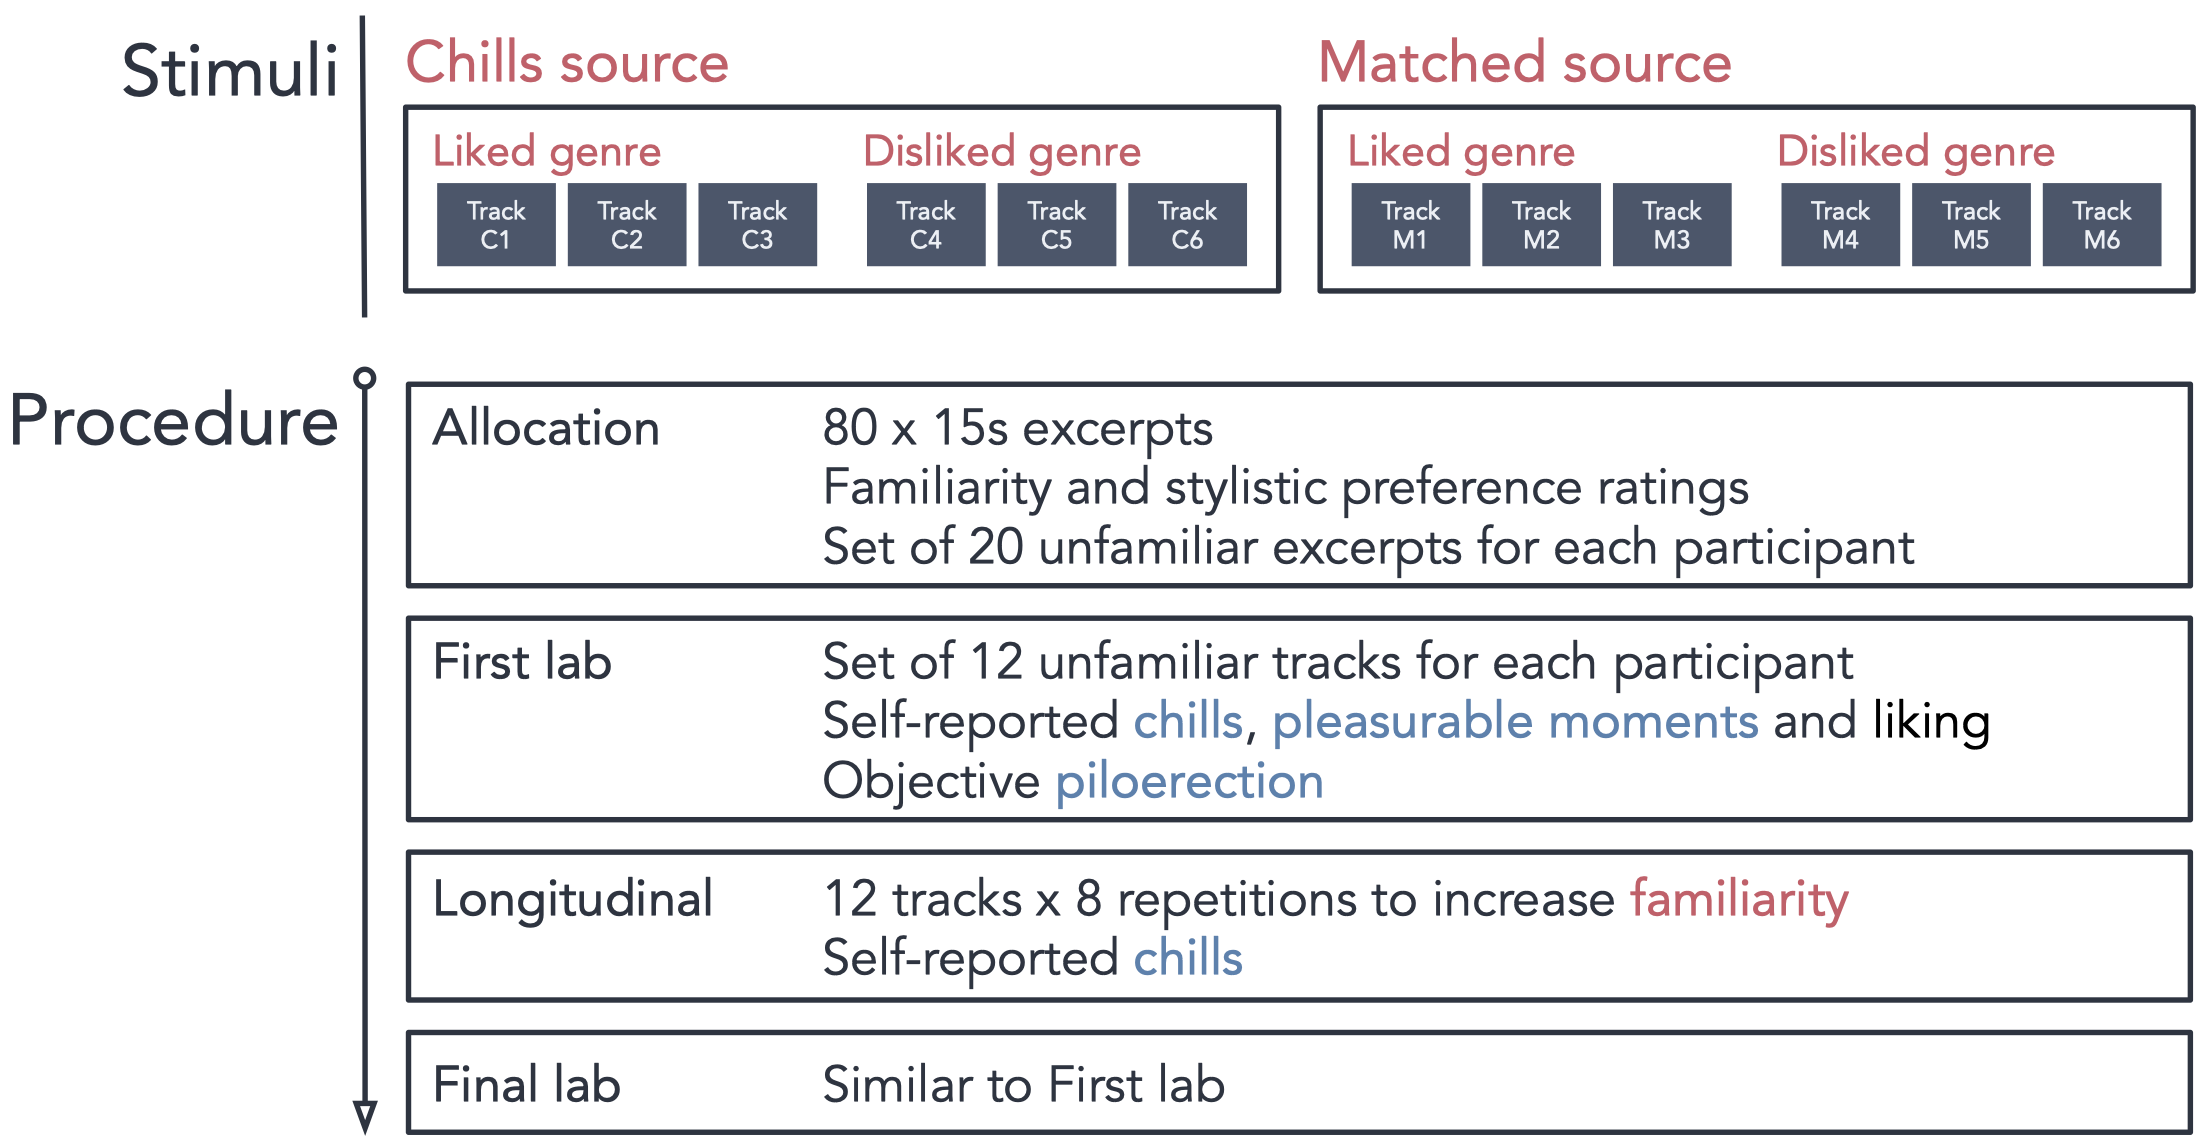
\includegraphics[width=\textwidth]{con-5.png}
\centering
\caption{Simplified summary of the experimental design. The main independent variables are shown in red, and the main dependent variables are shown in blue.}
\label{fig:con-5}
\end{figure}

\section{Analysis}

\subsection{Piloerection data}

Video file processing was automated using FFmpeg \parencite{tomar2006}, an open-source command-line tool for handling multimedia files. Due to the long duration of the lab session, the footage was split into multiple files when saved to the GoPro's SD card. Using FFmpeg, the files were concatenated into a single, large video file per session. Synchronisation between the video and the experiment logs was achieved by careful manual identification of the timestamp at which the Goosecam's green LED light and piezo buzzer first switched on, signifying that the serial message for the first baseline recording had just been received, and by trimming the video before that timestamp. The skin-side cutout was centred and cropped down to 506 $\times$ 506 px to ensure only an illuminated portion of the skin would be captured. The video was then rotated by 90º to reach the expected orientation (due to the way the GoPro had to be mounted on the Goosecam), audio signal was removed from the file, and the frame rate was downsampled to 10 Hz. Finally, the video was automatically split into individual files corresponding to each track, using the timestamps logged by the lab session platform.

Individual video files were processed with Gooselab,\footnote{The official link to the Gooselab toolbox is deprecated, and currently, there seems to be no official repository for the toolbox but luckily, a working version was found on Github: \url{https://github.com/tstenner/gooselab}} a MATLAB toolbox which performs the computations described in Benedek et al's (\citeyear{benedek2010}) article. Broadly speaking, for each frame, the toolbox extracted the largest possible square image from the video file (an unnecessary step in this case, since the frames had already been cropped), before converting it to grey scale, applying a high-pass filter, running a two-dimensional discrete Fourier transform, performing angular averaging, and computing piloerection as the maximum amplitude within a specific frequency range. This process resulted in a time-series showing piloerection values for each frame, with higher values corresponding to greater observed piloerection.

Piloerection events then needed to be extracted from these continuous time-series. To do so, for each combination of lab session, participant, and track, a threshold was set at three standard deviations over the average baseline value. Piloerection events for each track were then assigned to each period of at least ten consecutive frames (i.e., one second) exceeding that threshold value, with the onset and offset of piloerection occurring on the first and last frame the threshold was exceeded for that event, following the updated recommendations by \textcite{benedek2011}. \autoref{fig:con-6} shows a particularly clear episode of piloerection, overlapping with self-reported MECs and pleasure.

\begin{figure}[t!]
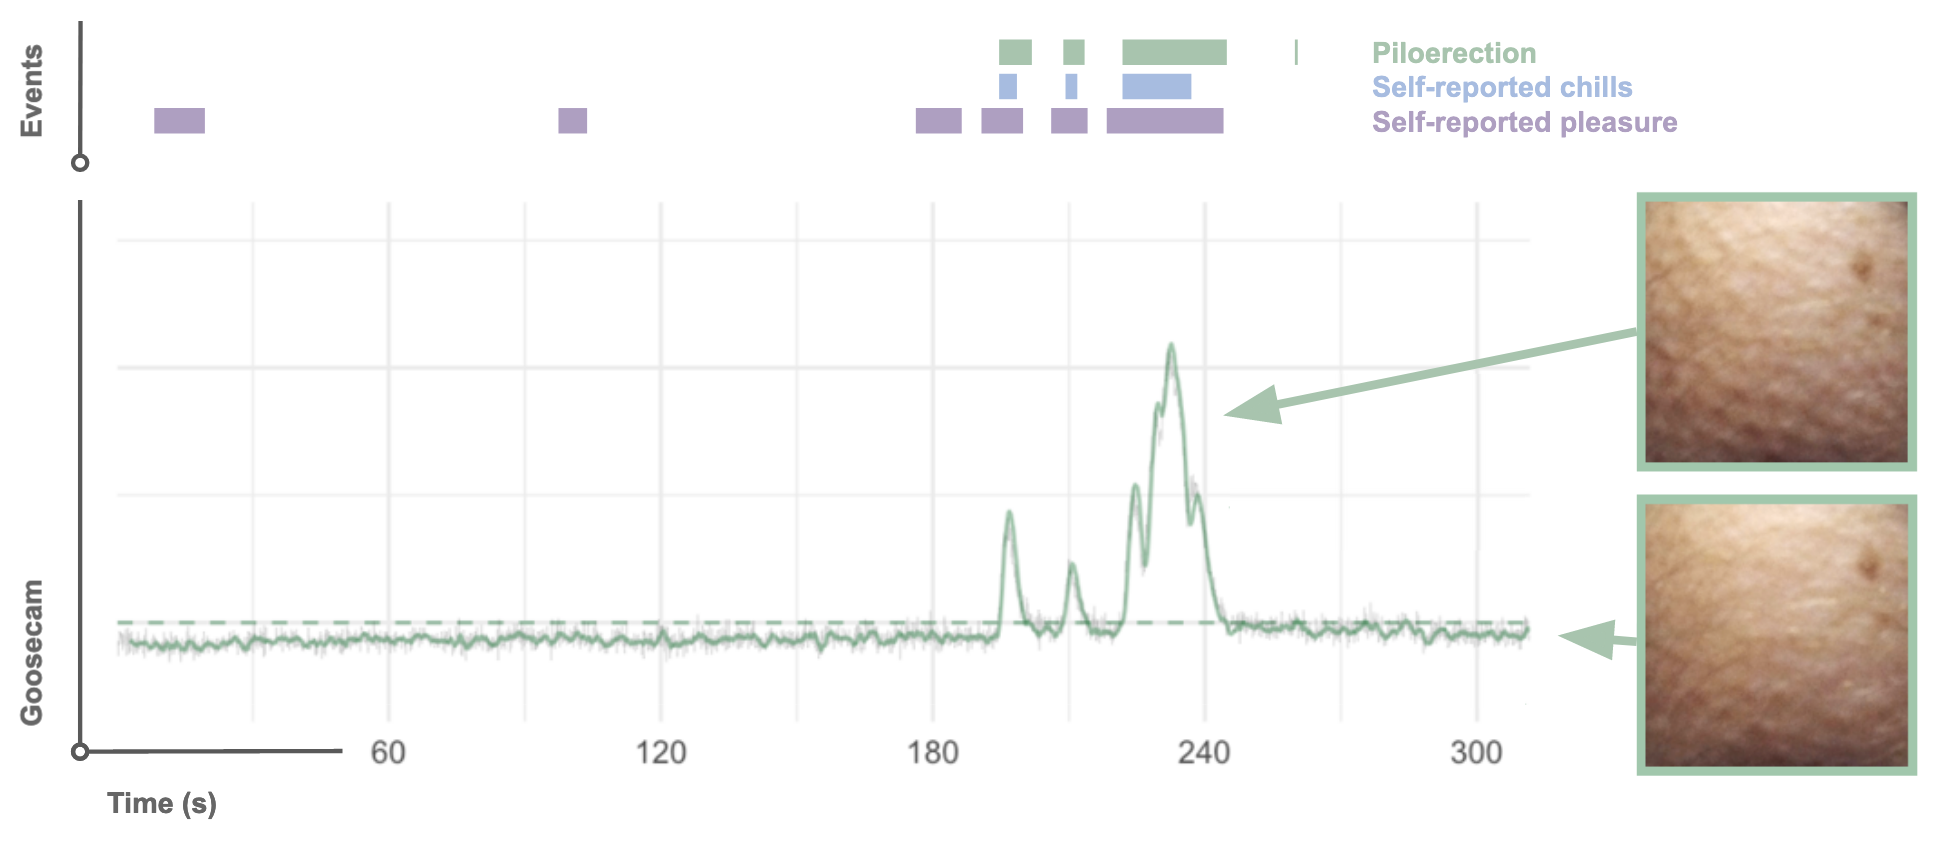
\includegraphics[width=\textwidth]{con-6.png}
\centering
\caption{Time-series of piloerection values. The threshold for a piloerection event to occur is indicated by the green dashed line. Raw piloerection values are shown faintly in grey, and smoothed values in green, for visualisation purposes only. If piloerection values exceeded the threshold for ten consecutive frames, a piloerection event was assigned to the track, as indicated by the green bar. In this case, the piloerection events considerably overlapped with self-reported MECs, in blue, and pleasure, in purple. Example video frames are shown at two different time points, displaying piloerection in the top frame, and no piloerection in the bottom frame.}
\label{fig:con-6}
\end{figure}

\subsection{Statistical analyses}

After data processing, the three dependent variables (MECs, piloerection, pleasure) consisted of time-series of binary events. There were several possibilities with regard to quantifying their occurrence within each track. For the first set of analyses, we opted to sum the duration of each event for each track, and to scale that value according to track duration, so as to not penalise slightly shorter tracks. The resulting value can be interpreted as the total duration (in seconds) for which events (e.g., MECs) were experienced during a track, if that track were five minutes long. This approach was chosen instead of simply counting tracks during which events occurred or not, since most tracks featured reports of MECs and pleasure, as later explained in the results, which would have resulted in a loss of much of the signal in the data. Another option would have been to simply count the number of events per track, but this would have been biased by small imprecisions in the measurements, such as long events being interrupted by the self-report key not being pressed properly for a short moment, or by piloerection values dipping below the threshold for just a few frames, for instance. Summing up the duration of events seemed like a reasonable compromise to keep as much of the signal as possible while minimising the risk for bias. Note that for these analyses, the resulting variable for piloerection was log-transformed in order to adhere to the assumptions of the statistical tests that were used.

For this first set of analysis, we fit a linear mixed-effects model for each of the dependent variables, using familiarity, stylistic preference, and source as fixed effects, and participant and track as random effects. We opted not to test for interaction effects due to the relatively large number of variables considering the small sample size, which would have increased the risk of overfitting the models. Since these models included all participants, regardless of whether or not they completed the longitudinal phase of the study, we also conducted paired t-test to test the effect of familiarity on each dependent variable for the subset of participants who attended both lab sessions. Finally, we fit another linear mixed-effect model to assess the extent to which the combination of all variables predicted the variance in the ratings of liking collected after listening to each track, therefore using MECs, piloerection, pleasure (all preprocessed by scaling the features, since they were continuous), familiarity, stylistic preference, and source as fixed effects, and participant and track as random effects. Note that for this analysis, the emphasis was placed on predictive power rather than interpretability, seeing as some of the variables were highly collinear.

All mixed-effects were fit using the \emph{lme4} R package \parencite{bates2015}. Diagnostic tests revealed that there were no high-leverage outliers, and that there was adequate homoscedasticity and normality of residuals (except for piloerection, at first, which is why the variable was eventually log-transformed). Model fits were evaluated by performing likelihood ratio tests, which were run by conducting ANOVAs comparing the fitted models with null models including random effects only. Marginal and conditional R\textsuperscript{2} values were obtained with the \emph{MuMIn} R package \parencite{barton2020}. Marginal R\textsuperscript{2} outlines the variance explained by the fixed effects only, while conditional R\textsuperscript{2} outlines the variance explained by the whole model \parencite{nakagawa2013}. Finally, p-values for the fixed effects were obtained using the \emph{lmerTest} R package \parencite{kuznetsova2017}.

To conclude the first set of analyses, a range of tests were conducted as sanity checks, as well as to explore some relationships in the data. First, we ran correlation tests to verify whether or not room temperature had an effect of the occurrence of piloerection and self-reports of MECs. Second, we ran a series of correlation tests and t-tests to test the existence of relationships between age, gender, and musical training and all of the dependent variables. Finally, we tested the correlations between the dependent variables themselves.

The second set of analyses concerned the longitudinal phase of the study, for which only occurrence of MECs at the track level was collected. Note that this data was analysed separately due to the completely different ways in which data was collected. While the longitudinal phase was mainly aimed at increasing familiarity for the final lab session, it also had the potential to reveal how repetition affected the occurrence of MECs. For this analysis, we fit a logistic mixed-effect model with number of repetitions as a fixed effect and participant, source, and stylistic preference as random effects. Apart from diagnostic tests on residuals, which are much less interpretable for logistic regression, the same procedures as detailed above were used to explain the model.

For the final set of analyses, the dependent variables were taken in their binary time-series form. The purpose of these analyses was to assess the degree of overlap between MECs, piloerection, and pleasure. For this purpose, permutation tests were chosen, as they allow for the convenience of choosing the most appropriate test statistic for the task at hand, and their nonparametric nature eliminates the need to validate many assumptions inherent to time-series analysis. A one-sided permutation test was run for each pair of dependent variables, using Monte Carlo estimation with 5000 replications. The test statistic was calculated by taking the percentage of frames during which both events occurred simultaneously, for each track, and then averaging the obtained values for each track over the whole experiment, resulting in an average rate of overlap per track. Permutations were conducted by randomly rearranging event onsets within each track, while ensuring that events did not overlap within a single variable. For example, if a given track was 20 seconds long, and contained two reports of MECs, from 0:05 to 0:07 and 0:11 to 0:16, a valid permutation for this variable would be to rearrange MECs so that they occur from 0:01 to 0:06 and from 0:17 to 0:19. However, rearranging MECs so that they occur from 0:01 to 0:06 and from 0:05 to 0:07 would not be valid, since these events overlap with each other.

\section{Results}

One participant displayed unusual patterns in their self-reported responses. After close inspection of their data, it appeared that the participant did not fully understand the task, and repeatedly pressed keys when MECs or pleasure occurred instead of keeping the keys pressed down as instructed, resulting not only in many more key strokes than any other participant, but also in small bugs due to the speed at which data was being written by OpenSesame while running the task. Instead of manually fixing the data, which would have required making a lot of assumptions as to what was the intended behaviour, we deemed it more appropriate to exclude this participant from the data analysis.

Of the remaining 29 participants, 27 reported MECs at least once, 11 experienced piloerection at least once, and all of them reported pleasure at least once. When looking at data at the track level, out of the 152 tracks that were listened to throughout the experiment, 116 caused MECs at least once, 32 for piloerection, and 135 for pleasure. Overall, using the scaled measure for the dependent variables (i.e., total duration per track if each track were five minutes long), MECs were experienced 20.8 seconds per track on average, 3.10 seconds for piloerection, and 46.0 seconds for pleasure.

\subsubsection{Effects of source, stylistic preference, and familiarity}

For MECs, the linear mixed-effects model yielded a significant fit ($\chi^2(3) = 36.84$, $p < .001$, $R^2_m = .047$, $R^2_c = .502$), revealing significant effects on MECs for familiarity ($b = 8.23$, $p = .013$), stylistic preference ($b = 15.47$, $p < .001$), but not source ($b = 4.80$, $p = .123$), with average reports of MECs increasing by 9.6 seconds for familiar tracks, and by 15.4 seconds for tracks in a liked genre. 

For log-transformed piloerection, the linear mixed-effect model yielded a significant fit ($\chi^2(3) = 11.35$, $p = .010$, $R^2_m = .017$, $R^2_c = .436$), revealing significant effects on piloerection for familiarity ($b = -0.19$, $p = .013$), stylistic preference ($b = 0.14$, $p = .031$), but not source ($b = -0.06$, $p = .394$), with average detected piloerection decreasing by 4.0 seconds for familiar tracks, and increasing by 2.75 seconds for tracks in a liked genre. 

For pleasure, the linear mixed-effects model yielded a significant fit ($\chi^2(3) = 65.43$, $p < .001$, $R^2_m = .088$, $R^2_c = .527$), revealing a significant effects on pleasure for stylistic preference ($b = 37.42$, $p < .001$), but not familiarity ($b = -0.43$, $p = .931$) or source ($b = 2.46$, $p = .599$), with average reports of pleasure increasing by 39.3 seconds for tracks in a liked genre.

Considering the large differences between marginal and conditional R\textsuperscript{2} in each model, simple linear regression models were also run to assess the individual contributions of participant ID and track ID to the variance in the dependent variables, revealing that, on their own, participants explain 45\% of the variance in MECs, 30\% in piloerection, and 38\% in pleasure, and tracks explain 10\%, 18\%, and 21\% respectively, as measured by the adjusted R\textsuperscript{2} of the fitted models.

Restricting the analysis only to the participants who completed both lab sessions, paired t-tests revealed a significant effect of familiarity (\emph{U} for \emph{unfamiliar}, \emph{F} for \emph{familiar} in the reported summary statistics) on MECs ($t(148) = 2.14$, $p = .034$, $M_U = 20.31$, $SD_U = 42.34$, $M_F = 28.50$, $SD_F = 52.46$) and piloerection ($t(148) = -2.11$, $p = .037$, $M_U = 4.38$, $SD_U = 23.03$, $M_F = 0.40$, $SD_F = 2.96$), but not on pleasure ($t(148) = -0.08$, $p = .937$, $M_U = 44.63$, $SD_U = 62.15$, $M_F = 44.29$, $SD_F = 57.52$), confirming the results from the mixed-effects models. For those participants, familiarity increased average reports of MECs by 8.2 seconds, and decreased detected piloerection by 4.0 seconds, consistently with the previous analyses.

\subsubsection{Combined effects on liking}

For liking, the linear mixed-effects model yielded a significant fit ($\chi^2(6) = 328.42$, $p < .001$, $R^2_m = .505$, $R^2_c = .709$), revealing significant effects on the ratings of liking collected after listening to each track for continuously reported pleasure ($b = 0.91$, $p < .001$) and stylistic preference ($b = 1.90$, $p < .001$), but not for the other variables, although it is worth keeping in mind that these individual effects are not interpretable, due to the high collinearity between some of the predictors.

\subsubsection{Sanity checks}

Room temperature was 21.2ºC on average (\emph{SD} = 1.9ºC), which is comparable to other studies which reported temperature \parencite{benedek2011,laeng2016}, and was not correlated with either MECs ($r(35) = -0.06$, $p = .711$) or piloerection ($r(35) = -0.09$, $p = .599$).

Age, gender, and musical training had no effect on any of MECs, piloerection, and pleasure (all $p > .05$), with gender (\emph{F} for \emph{female}, \emph{M} for \emph{male} in the reported summary statistics) trending the closest to significance, as seen with t-tests on MECs ($t(18.16) = 1.87$, $p = .077$, $M_F = 9.98$, $SD_F = 18.15$, $M_M = 29.65$, $SD_M = 33.59$), piloerection ($t(13.68) = -1.48$, $p = .163$, $M_F = 6.23$, $SD_F = 13.56$, $M_M = 0.81$, $SD_M = 2.12$), and pleasure ($t(20.03) = 1.88$, $p = .074$, $M_F = 34.06$, $SD_F = 30.76$, $M_M = 63.72$, $SD_M = 48.61$).

\subsubsection{Effect of repeated listening}

For the effect of repeated listening on MECs, the logistic mixed-effects model did not reach a significant fit ($\chi^2(1) = 1.92$, $p = .166$, $R^2_{m\Delta} = .001$, $R^2_{c\Delta} = .263$), and there was no significant effect ($b = 0.06$, $p = .16$), presumably due to high variance resulting from low sample size, as seen in \autoref{fig:con-7}.

\begin{figure}[t!]
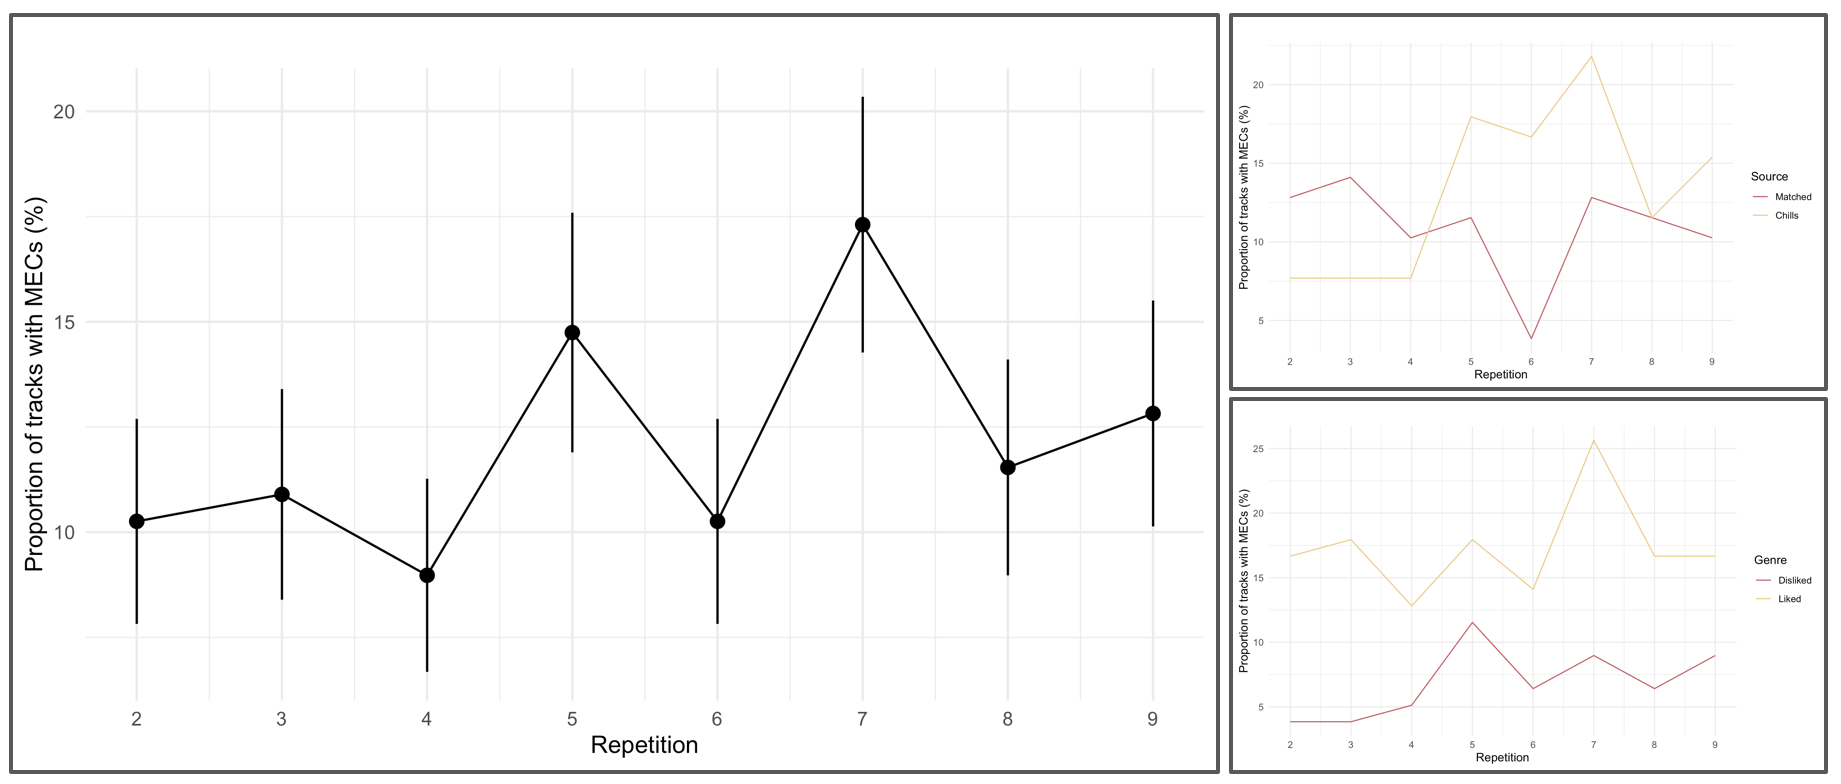
\includegraphics[width=\textwidth]{con-7.png}
\centering
\caption{Effect of repeated listening on the occurrence of self-reported MECs during the longitudinal phase of the study, starting from the second to the ninth repetition (the first and last repetitions occurring during the lab sessions, and therefore not shown or analysed). The first plot shows what might look like a slight overall increase over time, but with large day-to-day swings and high variance, as shown by the error bars. The two smaller plots show the differences in occurrence of MECs when tracks are split by source or stylistic preference, demonstrating that no clear patterns emerged other than that of tracks in liked genres causing more MECs than in disliked genres overall.}
\label{fig:con-7}
\end{figure}

\subsubsection{Relationships between dependent variables}

Correlation tests showed that average event durations were not correlated between piloerection and either of MECs ($r(491) = -0.02$, $p = .658$) or pleasure ($r(491) = 0.01$, $p = .827$), but that they were correlated between MECs and pleasure ($r(491) = 0.52$, $p < .001$).

When taken as binary time-series, however, these three variables showed highly significant overlaps, as shown by one-sided permutation tests using Monte Carlo estimation with 5000 replications. On average, the number of frames showing overlap between both responses represented 0.11\% of the total frames in the track for MECs and piloerection ($p < .001$), 3.26\% for MECs and pleasure ($p < .001$), and 0.16\% for piloerection and pleasure ($p < .001$). It should be noted that these effects seem small in magnitude because overlapping frames were compared to the total number of frames in all tracks. The permutation tests revealed that this degree of overlap was much greater than what would be expected by chance.

\section{Discussion}

In this study, we investigated the effects of musical content, stylistic preference, and familiarity on the occurrence of MECs, piloerection, and pleasure, by setting up a controlled, longitudinal experiment, ensuring that adequate comparisons could be drawn across all variables.

First, we observed that the majority of participants reported MECs and pleasure throughout the experiment, but than less than half of them experienced detectable piloerection. This represent an unusually high proportion of MECs \parencite[see Chapter \ref{ch:2} for a discussion about prevalence in experimental contexts, e.g.,][]{colver2016, grewe2009a, konecni2007b}, which could be explained by the fact that each phase of the study required a lot of music listening, and that the study itself was particularly long. In addition, participants were recruited based on their ability to often experience MECs, and tracks were selected to maximise the occurrence of MECs, or closely match tracks that do. Conversely, it could be argued that the duration and format of the experiment encouraged participants to overly report MECs. For instance, a participant could find it unusual to listen to twelve or more full tracks during an experiment while sitting in front of a keyboard and doing nothing at all, if they didn't experience MECs. This concern is slightly alleviated by the fact that, when they were reported, MECs did significantly overlap with piloerection, which is not consciously controlled by the participants.

The fact that participants experienced much fewer episodes of piloerection suggests a disconnect between reported MECs and piloerection. While there are arguments that piloerection might only occur beyond a specific MEC intensity threshold \parencite{sumpf2015}, other explanations could be that current piloerection detection methods are not yet accurate enough, or that piloerection and MECs are not mutually exclusive. It is difficult to determine from this study alone which of the responses is a more reliable indicator of MECs in general. More research is needed on the exact relationship between self-reported MECs and piloerection, and the methods introduced in this chapter might help in conducting such research. For the present study, however, this discrepancy between MECs and piloerection needs to be taken into consideration when interpreting the results discussed below.

Stylistic preference had a positive effect on all three of MECs, piloerection, and pleasure, which is not particularly surprising when it comes to pleasure, since we would expect more pleasure to be experienced when listening to music in liked genres. However, the fact that stylistic preference also drove the occurrence of MECs and piloerection suggests that the conflicting results in previous research \parencite{bannister2018, nusbaum2011} might have been due to inadequate research methods. In other words, rather than preference for specific genres (as identified by STOMP, for instance) leading to more MECs being experienced, it could be that it was the interaction between a listener's stylistic preferences and the music being listened to that had such an effect. This raises questions for future research about the role of stylistic knowledge or exposure. For instance, would MECs occur in liked but unfamiliar genres? The effects of stylistic preference and stylistic knowledge might be independent, or one could be mediated by the other, such as stylistic knowledge leading to stylistic preference, and in turn, stylistic preference increasing the likelihood of MECs, for instance. Further systematic study could help in this regard, and could potentially uncover valuable information about the role of expectation in the experience of MECs.

More surprisingly, familiarity had opposite effects on MECs and piloerection, and no effect on pleasure. These results were confirmed when only looking at the cohort of users who completed the longitudinal phase of the study. Pleasure remaining stable with repeated exposure goes against previous longitudinal findings that familiarity increases liking and music preference \parencite{chmiel2019,madison2017}. However, in the context of this study, pleasure was disproportionately higher for tracks in liked genres than for those in disliked genres. Pleasure could therefore have reached extreme values at the beginning of the study, and remained stable in time. We would also argue that pleasure is a more intense subjective response than liking or preference, and as such, might evolve more slowly over time. The opposite effects of familiarity on MECs and piloerection is interesting, and suggests, once again, fundamental differences between the two responses. One possible interpretation is that piloerection is more reliant on physiological processes and might be more subject to habituation as a result. Or it could be that the quantity of MECs increases with repeated exposure, but their intensity decreases, therefore not exceeding the threshold for piloerection discussed earlier. Leveraging the framework identified in Chapter \ref{ch:2}, these results could also suggest that MECs which involve piloerection rely on different psychological and evolutionary mechanisms than those which don't. Some MECs based on personal meaning could therefore benefit from repeated exposure, while others based on surprise could temporarily disappear due to frequent listening.

Musical content, manipulated via stimulus source, had no effect whatsoever. As will be discussed more extensively in Chapter \ref{ch:4}, it could be the result of the strict matching procedure, i.e., an effect might have been detected by randomly sampling control tracks from any artist and level of popularity instead. Since it is fundamentally impossible to know if tracks from the matched source can cause MECs or not (in all likelihood, some of them can), it could be that, by applying a strict matching procedure, the features which cause MECs were present to the same extent in the chills and matched sources. The assumption behind the manipulation of stimulus source was that, if an effect of musical content exists, it should be detectable in aggregate because some stimulus-driven properties would make tracks from the chills source slightly more likely to cause MECs for several individuals.

Additional context comes from the fact that the models discussed so far all featured high conditional R\textsuperscript{2} values, and low marginal R\textsuperscript{2} values. This suggests that, while the results presented so far were indeed significant, they accounted for a small proportion of the variance in the dependent variables. Conversely, on their own, participants and tracks accounted for much variance in the outcomes, which indicates that participants have predictable response patterns, and that specific tracks tend to elicit similar responses. The former might be explained by individual differences, or simply by differences in how participants understood the task or decided what passes the threshold of reporting MECs or pleasure. Alternatively, the large number of tracks with no recorded response at all might on its own account for much of these conditional R\textsuperscript{2} values.

Regardless, in the context of this study, it appears that likelihood of detecting an effect of musical content was overestimated, especially if MECs partly rely on personal meaning and not on stimulus-based elicitors, which would lead to ceiling effects. However, we do know through previous research \parencite[e.g.,][]{sloboda1991} that there is an effect of acoustic and musical elicitors. Considering the small effect sizes obtained in the present analyses, it becomes clear that this effect is subtle, and that much larger amounts of data would be needed to detect it. This is a type of problem that is particularly well suited to computational approaches, and that will be the main subject of the rest of this thesis.

As opposed to the models discussed so far for continuous self-reports of MECs, piloerection, and pleasure, effect sizes for both the fixed effects and the whole model itself were large with regard to static ratings of liking collected after listening to each track, with source, stylistic preference, familiarity, MECs, piloerection, and pleasure accounting for about 50\% of the variance in self-reported liking for tracks. While further analysis, and probably a different study design, would be needed to fully disentangle the individual contributions of these fixed effects, it is interesting that much of music preference can be predicted from a relatively small number of factors, and certainly suggests that preference could be even more accurately predicted in a study dedicated to this purpose.

As expected (see Chapter \ref{ch:2}), there were no effects of age, gender, or musical training on any of the dependent variables, but interestingly, there were some subtle differences due to gender, with female participants experiencing more piloerection but fewer MECs and less pleasure than male participants. Interpretation is limited here by the fact that these differences were non-significant, and that there is currently no convincing hypothesis as to why such differences would exist.

For repeated exposure, while the primary objective of making participants listen to the tracks between the two lab sessions was to increase familiarity, we did collect some data about the occurrence of MECs. No effect of repeated listening was detected, but a small upward trend was visible on the figure representing the proportion of MECs experienced over time. It is worth noting that for this phase of the study, sample size was relatively low, there was less control over experimental conditions, and MECs were reported in a different way. Such an investigation might reveal interesting insights if conducted as a larger study, but for the present study, the manipulation achieved the intended objective of increasing familiarity.

Finally, we observed correlations between MECs and pleasure, but neither of them were correlated with piloerection. However, permutation tests revealed significant overlaps for all three variables. In fact, the test statistics had the most extreme values out of all 5000 Monte Carlo simulations for all three pairs of variables, indicating that the degree of overlap between them was almost impossible to achieve by chance. This suggests that while piloerection differs from MECs and pleasure, it is still strongly related to both of these responses. In other words, they overlap significantly, but this doesn't mean that they overlap exclusively, which provides further support for the hypotheses that piloerection requires exceeding an activation threshold \parencite{sumpf2015}, or alternatively, that they only represent a subset of MECs and pleasurable moments in music. A potential caveat is that the overlap between MECs and pleasure could be driven by asking participants to self-report the two measures at the same time, using similar modalities. The mutual overlap with piloerection alleviates that concern to some extent, since piloerection was recorded using a device the participants had no control over, as discussed earlier.

Overall, there remain some unexplainable differences between MECs and piloerection, with many participants reporting MECs, but few experiencing piloerection. It could be that the Goosecam is at fault, but visual inspection of the video files did not result in the detection of any obvious sensor errors. When debriefing after the end of the experiment, several participants mentioned experiencing piloerection in the neck, as has already been identified in previous research \parencite[e.g.,][]{panksepp1995}. While it is difficult to imagine asking participants to wear the current iteration of the Goosecam around their neck, it would be helpful to eventually have access to better, more compact sensors, which could enable the simultaneous collection of piloerection data from different areas of the body. This is related to the difficulty in gaining confidence in participants' self-reports of MECs, given the large differences in reporting behaviours across participants. Perhaps subjective experiences of MECs are very different across individuals, but we suspect that instead, it is just particularly difficult to identify a definition of MECs that is not liable to subjective interpretation. Further efforts towards the development of accurate and objective detection methods for the overall experience of MECs, as opposed to piloerection only, would go a long way in furthering research on MECs.

This study achieved many of its stated objectives, identifying strong effects of stylistic preference on MECs, piloerection, and pleasure, opposite effects of familiarity on MECs and piloerection, high predictability of liking based on a small set of variables, and significant overlap between MECs, piloerection, and pleasure, highlighting the close links between MECs and emotional and aesthetic responses.

The investigated phenomena are complex, and differ highly across individuals, and yet, these effects were detected, despite understandably small effect sizes. The only exception is for musical content, which most likely requires much larger amounts of data. Approaches aiming to do so are detailed in the next two chapters of this thesis, starting in Chapter \ref{ch:4} with a corpus analysis of the relationship between valence and MECs.
